% Modelo actual de BCS: segmentador de regiones (DINOv2-B ajustado + FPN)
% + DINOv2-L congelado con promedio por región + ridge.
% Compilar: pdflatex modelo_bcs.tex
\documentclass[tikz,border=6pt]{standalone}
\usepackage[utf8]{inputenc}
\usepackage[T1]{fontenc}
\usepackage{amsmath}
\usetikzlibrary{positioning,arrows.meta,fit,backgrounds,calc}

\definecolor{ink}{HTML}{1F2A24}
\definecolor{paper}{HTML}{F6F4EE}
\definecolor{verde}{HTML}{2E6F57}
\definecolor{verdeclaro}{HTML}{E6EFE9}
\definecolor{cobre}{HTML}{A85A1C}
\definecolor{cobreclaro}{HTML}{F6E3D3}
\definecolor{gris}{HTML}{4D5A52}

\tikzset{
  font=\sffamily\small, >={Stealth[length=2.4mm]},
  caja/.style={draw=ink, line width=0.6pt, rounded corners=3pt, fill=white,
               align=center, minimum height=1.25cm, inner sep=5pt, text width=#1},
  caja/.default=2.8cm,
  ajustado/.style={caja=#1, fill=cobreclaro, draw=cobre},
  ajustado/.default=2.8cm,
  congelado/.style={caja=#1, fill=verdeclaro, draw=verde},
  congelado/.default=2.8cm,
  dato/.style={draw=gris, dashed, rounded corners=3pt, fill=paper, align=center,
               minimum height=1.0cm, inner sep=4pt, text width=#1, font=\sffamily\footnotesize},
  dato/.default=2.4cm,
  flecha/.style={->, line width=0.8pt, draw=ink},
  dim/.style={font=\sffamily\scriptsize, text=gris},
  rama/.style={draw=gris!60, rounded corners=6pt, inner sep=8pt, line width=0.5pt},
  etiq/.style={font=\sffamily\footnotesize\bfseries, text=gris, anchor=south west},
}

\begin{document}
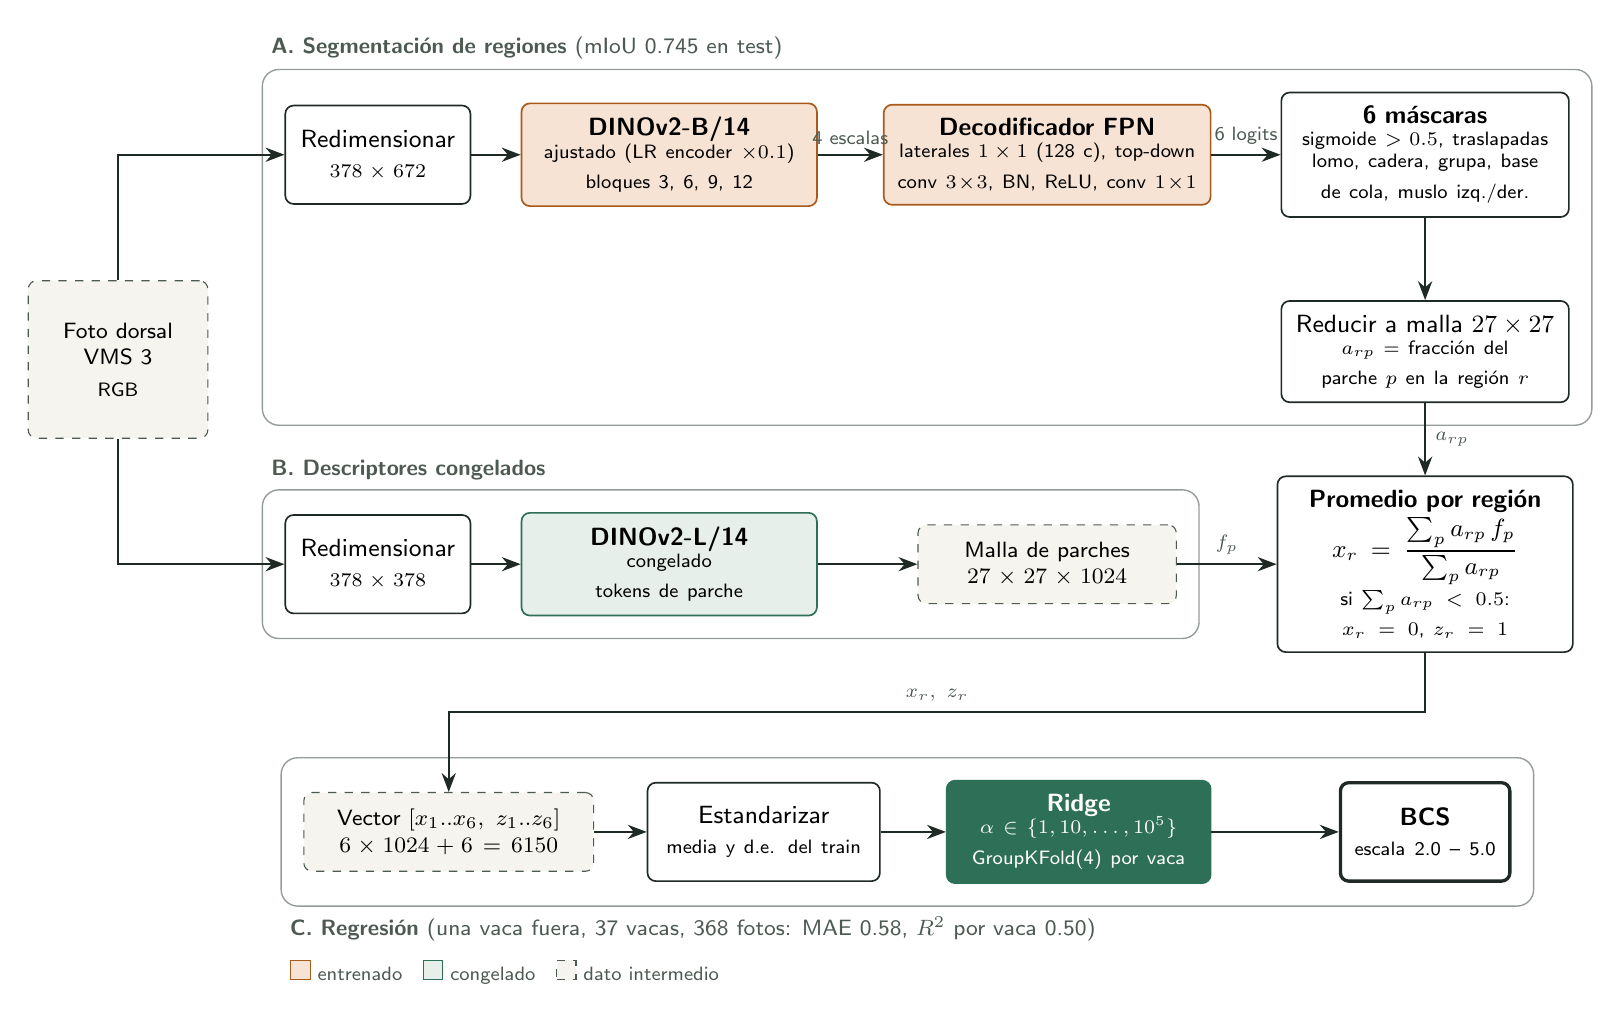
\begin{tikzpicture}[node distance=0.55cm and 0.55cm]

% ---------- Entrada ----------
\node[dato=2.0cm, minimum height=2.0cm] (img) at (0,-2.6) {Foto dorsal\\VMS 3\\[2pt]\scriptsize RGB};

% ---------- Rama A: segmentación de regiones ----------
\node[caja=2.0cm]     (rsA)   at (3.3,0)    {Redimensionar\\\scriptsize $378\times672$};
\node[ajustado=3.4cm] (encB)  at (7.0,0)    {\textbf{DINOv2-B/14}\\\scriptsize ajustado (LR encoder $\times0.1$)\\\scriptsize bloques 3, 6, 9, 12};
\node[ajustado=3.8cm] (dec)   at (11.8,0)   {\textbf{Decodificador FPN}\\\scriptsize laterales $1\times1$ (128 c), top-down\\\scriptsize conv $3\times3$, BN, ReLU, conv $1\times1$};
\node[caja=3.3cm]     (masks) at (16.6,0)   {\textbf{6 máscaras}\\\scriptsize sigmoide $>0.5$, traslapadas\\\scriptsize lomo, cadera, grupa, base\\\scriptsize de cola, muslo izq./der.};
\node[caja=3.3cm]     (grid)  at (16.6,-2.5) {Reducir a malla $27\times27$\\\scriptsize $a_{rp}$ = fracción del\\\scriptsize parche $p$ en la región $r$};

% ---------- Rama B: descriptores congelados ----------
\node[caja=2.0cm]      (rsB)  at (3.3,-5.2)  {Redimensionar\\\scriptsize $378\times378$};
\node[congelado=3.4cm] (encL) at (7.0,-5.2)  {\textbf{DINOv2-L/14}\\\scriptsize congelado\\\scriptsize tokens de parche};
\node[dato=3.0cm]      (tok)  at (11.8,-5.2) {Malla de parches\\$27\times27\times1024$};

% ---------- Fusión ----------
\node[caja=3.4cm] (map) at (16.6,-5.2) {\textbf{Promedio por región}\\[1pt]
  $\displaystyle x_r=\frac{\sum_p a_{rp}\,f_p}{\sum_p a_{rp}}$\\[1pt]
  \scriptsize si $\sum_p a_{rp}<0.5$: $x_r=0$, $z_r=1$};

% ---------- Regresión ----------
\node[dato=3.4cm] (vec) at (4.2,-8.6) {Vector $[x_1..x_6,\ z_1..z_6]$\\$6\times1024+6=6150$};
\node[caja=2.6cm] (std) at (8.2,-8.6) {Estandarizar\\\scriptsize media y d.e. del train};
\node[caja=3.0cm, fill=verde, text=white, draw=verde] (ridge) at (12.2,-8.6) {\textbf{Ridge}\\\scriptsize $\alpha\in\{1,10,\dots,10^5\}$\\\scriptsize GroupKFold(4) por vaca};
\node[caja=1.8cm, line width=1.2pt, font=\sffamily\small\bfseries] (bcs) at (16.6,-8.6) {BCS\\\scriptsize\mdseries escala 2.0 -- 5.0};

% ---------- Flechas ----------
\draw[flecha] (img.north) |- (rsA.west);
\draw[flecha] (img.south) |- (rsB.west);
\draw[flecha] (rsA) -- (encB);
\draw[flecha] (encB) -- node[dim, above]{4 escalas} (dec);
\draw[flecha] (dec) -- node[dim, above]{6 logits} (masks);
\draw[flecha] (masks) -- (grid);
\draw[flecha] (grid) -- node[dim, right]{$a_{rp}$} (map);
\draw[flecha] (rsB) -- (encL);
\draw[flecha] (encL) -- (tok);
\draw[flecha] (tok) -- node[dim, above]{$f_p$} (map);
\draw[flecha] (map.south) -- ++(0,-0.75) -| node[dim, pos=0.25, above]{$x_r,\ z_r$} (vec.north);
\draw[flecha] (vec) -- (std);
\draw[flecha] (std) -- (ridge);
\draw[flecha] (ridge) -- (bcs);

% ---------- Marcos ----------
\begin{scope}[on background layer]
  \node[rama, fit=(rsA)(encB)(dec)(masks)(grid)] (ramaA) {};
  \node[rama, fit=(rsB)(encL)(tok)] (ramaB) {};
  \node[rama, fit=(vec)(std)(ridge)(bcs)] (ramaC) {};
\end{scope}
\node[etiq] at (ramaA.north west) {A. Segmentación de regiones \textmd{(mIoU 0.745 en test)}};
\node[etiq] at (ramaB.north west) {B. Descriptores congelados};
\node[etiq, anchor=north west] at (ramaC.south west) {C. Regresión \textmd{(una vaca fuera, 37 vacas, 368 fotos: MAE 0.58, $R^2$ por vaca 0.50)}};

% ---------- Leyenda ----------
\node[anchor=north west, font=\sffamily\scriptsize, text=gris] at ($(ramaC.south west)+(0,-0.55)$) {%
  \tikz\node[fill=cobreclaro, draw=cobre, minimum size=7pt, inner sep=0]{}; entrenado\quad
  \tikz\node[fill=verdeclaro, draw=verde, minimum size=7pt, inner sep=0]{}; congelado\quad
  \tikz\node[fill=paper, draw=gris, dashed, minimum size=7pt, inner sep=0]{}; dato intermedio};

\end{tikzpicture}
\end{document}
